\documentclass[12pt,a4paper]{article}
\usepackage[T1]{fontenc}
\usepackage[francais]{babel}
\usepackage{graphicx}
\usepackage{url}
\usepackage{tabularx}
\usepackage{hyperref}
\usepackage{lmodern}
\usepackage[margin=2.5cm]{geometry}

\title{Rapport - Plateforme de Streaming Vidéo}
\author{Chamas Majd}
\date{\today}

\begin{document}

% Page de garde
\begin{titlepage}
\centering

\includegraphics[width=0.4\textwidth]{logo8.png}\par
\vspace{1cm}
{\Huge\bfseries Rapport\par}
{\LARGE Plateforme de Streaming Vidéo "BING"\par}
\vspace{2cm}

{\Large Chamas Majd\par} % Remplacer ici
\vfill
{\large \today\par}
\end{titlepage}

% Table des matières
\tableofcontents
\newpage

%-------------------------------------------------------
\section{Introduction}
\subsection{Présentation du projet}
Le projet consiste en une plateforme de streaming vidéo nommée "BING" permettant :
\begin{itemize}
\item De regarder des films et séries en ligne
\item De gérer plusieurs profils utilisateurs
\item De souscrire à des abonnements (Basic, Standard, Premium)
\item D'ajouter des vidéos en favoris
\end{itemize}

%-------------------------------------------------------
\section{Structure du site}
\subsection{Pages principales}
\begin{itemize}
\item \textbf{Accueil} : Affiche les contenus populaires et les suggestions
\item \textbf{Films/Séries} : Liste organisée par catégories
\item \textbf{Lecture vidéo} : Lecteur intégré avec informations
\item \textbf{Compte} : Gestion des abonnements et profils
\item \textbf{Inscription} : Choix d'un plan et paiement
\end{itemize}

%-------------------------------------------------------
\section{Base de données}
\subsection{Description}
\begin{itemize}
\item \textbf{Utilisateur} : Informations des comptes
\item \textbf{Video} : Métadonnées des contenus
\item \textbf{Favorites} : Association utilisateurs-contenus
\item \textbf{Abonnement} : Détails des plans
\end{itemize}

\begin{figure}[htbp]
\centering
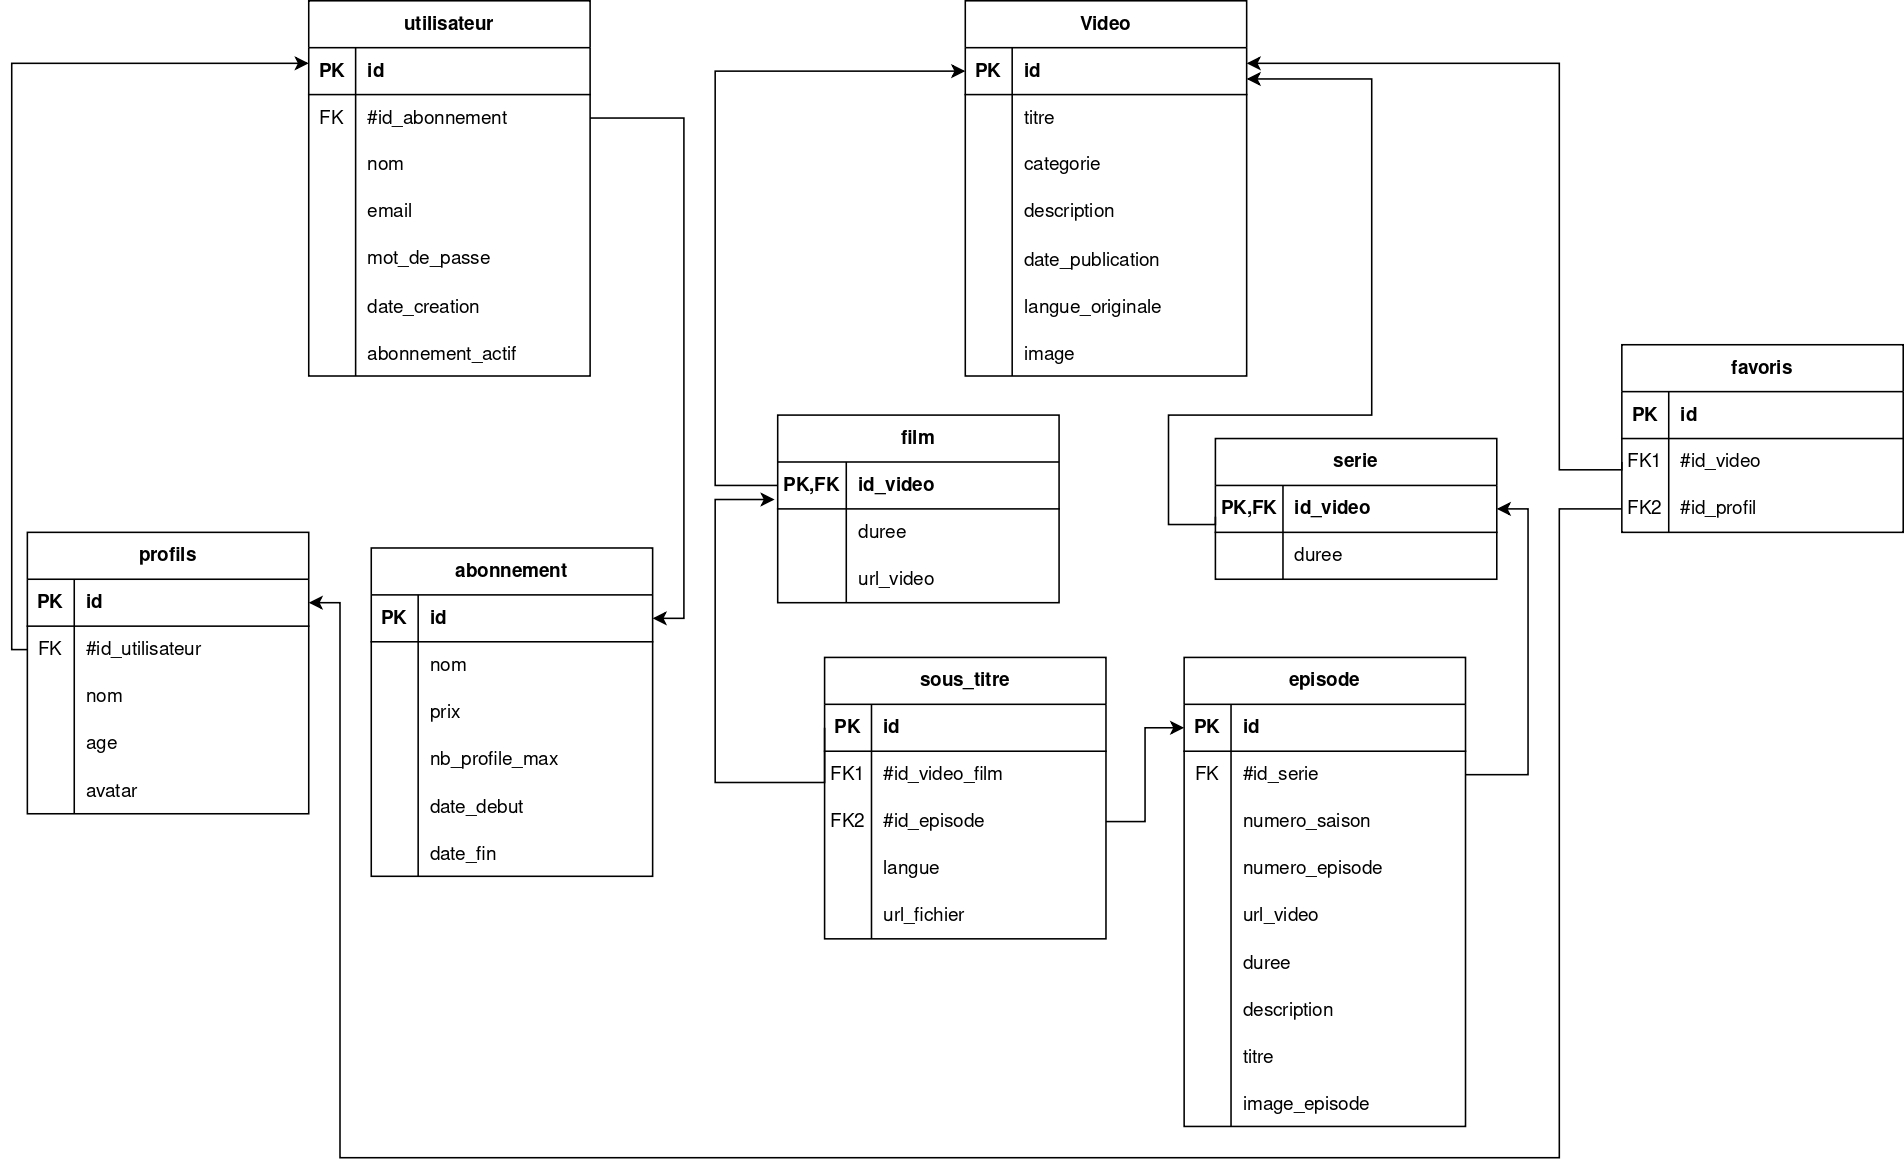
\includegraphics[width=1\textwidth,height=0.7\textheight,keepaspectratio]{schema.jpg}
\caption{Schéma complet de la base de données}
\label{fig:schema}
\end{figure}

%-------------------------------------------------------
\section{Fonctionnalités importantes}
\subsection{Gestion des comptes}
\begin{itemize}
\item Jusqu'à 5 profils par compte
\item Changement de mot de passe sécurisé
\item Favoris individuels par profil
\end{itemize}

\subsection{Abonnements}
\begin{itemize}
\item 3 plans avec avantages différents :
  \begin{itemize}
  \item Basic : 1 profil, qualité HD
  \item Standard : 3 profils, qualité Full HD
  \item Premium : 5 profils, qualité 4K
  \end{itemize}
\item Page de paiement simulé
\item Gestion automatique des profils
\end{itemize}

%-------------------------------------------------------
\section{Difficultés rencontrées}
\subsection{Changement d'abonnement}
\begin{itemize}
\item Calcul complexe des différences de prix
\item Gestion des profils excédentaires
\item Suppression automatique des anciens profils
\end{itemize}

Exemple concret : 
\begin{enumerate}
\item Utilisateur Premium (5 profils) → Basic (1 profil)
\item Suppression des 4 profils les plus anciens
\item Blocage de la création de nouveaux profils
\end{enumerate}

%-------------------------------------------------------
\section{Améliorations possibles}
\begin{itemize}
\item Ajout d'un vrai système de paiement (Stripe)
\item Téléchargement de vidéos hors ligne
\item Recommandations basées sur l'IA
\item Internationalisation (multi-langues)
\item Sous-titres multilingues
\end{itemize}

%-------------------------------------------------------
\section{Technologies utilisées}
\begin{itemize}
\item PHP pour la logique métier
\item HTML/CSS pour l'interface
\item JavaScript pour l'interactivité
\item SQLITE pour la base de données
\end{itemize}

\end{document}